% Composition: SV path (top, compact) + MLP-residual path (bottom) -> "+".
%   top:    d ──► [SC] ──► ⬭      (entire chain fits inside MLP width)
%                                            ▼
%                                           (+)
%                                            ▲
%   bot:    [feature stack] ──► MLP ── residual ──┘
\documentclass[tikz,border=4pt]{standalone}
\usepackage{tikz}
\usepackage{xcolor}
\usepackage{libertine}              % Linux Libertine (SIGGRAPH body font)
\usepackage[libertine]{newtxmath}    % matching math (provides AMS symbols)
\usepackage{amsmath}
\usetikzlibrary{positioning, calc, arrows.meta}

\begin{document}
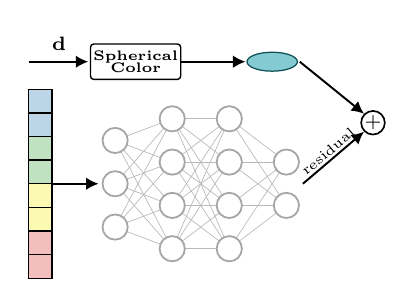
\begin{tikzpicture}[
  font=\sffamily\footnotesize,
  >={Latex[length=4.5pt,width=4.5pt]},
]

\definecolor{cBlue} {HTML}{1F77B4}
\definecolor{cGreen}{HTML}{2CA02C}
\definecolor{cLemon}{HTML}{F4ED00}
\definecolor{cRedB} {HTML}{D62728}
\definecolor{cCyan} {HTML}{1F9FAE}

% =====================================================================
% Feature column (left, bottom path)
% =====================================================================
\pgfmathsetmacro{\fw}{0.30}
\pgfmathsetmacro{\fxL}{0.00}
\pgfmathsetmacro{\fxR}{\fxL + \fw}
\pgfmathsetmacro{\fyTop}{1.20}

\foreach \i/\col in {0/cBlue, 1/cBlue,
                      2/cGreen, 3/cGreen,
                      4/cLemon, 5/cLemon,
                      6/cRedB,  7/cRedB}{
  \pgfmathsetmacro{\fyHi}{\fyTop - \i*\fw}
  \pgfmathsetmacro{\fyLo}{\fyHi - \fw}
  \fill[\col!30!white] (\fxL,\fyLo) rectangle (\fxR,\fyHi);
  \draw[black, line width=0.5pt] (\fxL,\fyLo) rectangle (\fxR,\fyHi);
}

% =====================================================================
% MLP (bottom path)
% =====================================================================
\pgfmathsetmacro{\mlpOx}{1.10}
\pgfmathsetmacro{\xA}{\mlpOx + 0.000}
\pgfmathsetmacro{\xB}{\mlpOx + 0.725}
\pgfmathsetmacro{\xC}{\mlpOx + 1.450}
\pgfmathsetmacro{\xD}{\mlpOx + 2.175}
\pgfmathsetmacro{\vs}{0.55}
\pgfmathsetmacro{\nr}{0.16}

\foreach \i [count=\k from 0] in {-1, 0, 1}                  { \coordinate (A\k) at (\xA, \i*\vs); }
\foreach \i [count=\k from 0] in {-1.5, -0.5, 0.5, 1.5}      { \coordinate (B\k) at (\xB, \i*\vs); }
\foreach \i [count=\k from 0] in {-1.5, -0.5, 0.5, 1.5}      { \coordinate (C\k) at (\xC, \i*\vs); }
\foreach \i [count=\k from 0] in {-0.5, 0.5}                 { \coordinate (D\k) at (\xD, \i*\vs); }

\foreach \a in {0,1,2}    {\foreach \b in {0,1,2,3} {\draw[gray!55, line width=0.25pt] (A\a) -- (B\b);}}
\foreach \a in {0,1,2,3}  {\foreach \b in {0,1,2,3} {\draw[gray!55, line width=0.25pt] (B\a) -- (C\b);}}
\foreach \a in {0,1,2,3}  {\foreach \b in {0,1}     {\draw[gray!55, line width=0.25pt] (C\a) -- (D\b);}}

\foreach \name in {A0,A1,A2, B0,B1,B2,B3, C0,C1,C2,C3, D0,D1}{
  \fill[white] (\name) circle (\nr);
  \draw[gray!70, line width=0.65pt] (\name) circle (\nr);
}

% feature → MLP
\draw[black, line width=0.7pt, ->]
  (\fxR, 0) -- (\xA - \nr - 0.05, 0);

% =====================================================================
% SV element on TOP — much smaller, contained within the MLP width.
% MLP visible x-range: [xA-nr, xD+nr] = [0.94, 3.435]  (≈ 2.50 cm wide)
% d starts at x=0 (aligned with feature column left edge).
% =====================================================================
\pgfmathsetmacro{\svy}{1.55}
\pgfmathsetmacro{\mlpLeft}{\xA - \nr}    % 0.94
\pgfmathsetmacro{\mlpRight}{\xD + \nr}   % 3.435

% d origin (aligned with feature column left side)
\coordinate (dStart) at (\fxL, \svy);

% SC box: very compact
\node[draw=black, line width=0.5pt, rounded corners=1.2pt,
      fill=white, minimum width=8mm, minimum height=4.5mm,
      align=center, inner sep=1pt,
      font=\rmfamily\bfseries\fontsize{4}{4.5}\selectfont]
      (scBox) at (\mlpLeft + 0.42, \svy) {Spherical\\Color};

% d → SC (small gap before the box, matching SC → cyan)
\draw[black, line width=0.6pt, ->]
  (dStart) -- ($(scBox.west) + (-0.02, 0)$);
\node[font=\sffamily\scriptsize, anchor=south]
  at ($(dStart)!0.5!(scBox.west) + (0, 0.02)$) {$\mathbf{d}$};

% Cyan ellipse (same x/y proportions as before: 0.85/0.32 ≈ 2.66:1)
\pgfmathsetmacro{\eXr}{0.32}                  % x radius
\pgfmathsetmacro{\eYr}{\eXr / 2.66}            % y radius (proportional)
\pgfmathsetmacro{\eCx}{\mlpRight - \eXr - 0.02}  % center x: right edge sits just inside MLP right
\coordinate (svSurfel) at (\eCx, \svy);

% SC → cyan (arrow touches the ellipse, as before)
\draw[black, line width=0.6pt, ->]
  (scBox.east) -- ($(svSurfel) + (-\eXr - 0.02, 0)$);

\begin{scope}[shift={(svSurfel)}]
  \filldraw[fill=cCyan!55!white, draw=cCyan!50!black, line width=0.45pt]
    (0,0) ellipse [x radius=\eXr, y radius=\eYr];
\end{scope}

% =====================================================================
% "+" merge operator
% =====================================================================
\pgfmathsetmacro{\plusX}{\xD + 1.10}
\pgfmathsetmacro{\plusY}{0.5*\svy}
\node[draw=black, line width=0.6pt, circle, inner sep=0pt,
      minimum size=3mm, fill=white,
      font=\sffamily\scriptsize] (plus) at (\plusX, \plusY) {$+$};

% cyan surfel → + (top input). Tiny gap so the arrow visually starts at the ellipse.
\draw[black, line width=0.7pt, ->]
  ($(svSurfel) + (\eXr + 0.03, 0)$) -- (plus.north west);

% MLP → "residual" → + (bottom input). Label sloped along the arrow.
\draw[black, line width=0.7pt, ->]
  (\xD + \nr + 0.05, 0) -- (plus.south west)
  node[pos=0.5, sloped, above, font=\rmfamily\fontsize{5}{6}\selectfont,
       inner sep=1pt]
  {residual};

\end{tikzpicture}
\end{document}
